\documentclass{book}
\usepackage[a4paper,top=2.5cm,bottom=2.5cm,left=2.5cm,right=2.5cm]{geometry}
\usepackage{makeidx}
\usepackage{natbib}
\usepackage{graphicx}
\usepackage{multicol}
\usepackage{float}
\usepackage{listings}
\usepackage{color}
\usepackage{ifthen}
\usepackage[table]{xcolor}
\usepackage{textcomp}
\usepackage{alltt}
\usepackage{ifpdf}
\ifpdf
\usepackage[pdftex,
            pagebackref=true,
            colorlinks=true,
            linkcolor=blue,
            unicode
           ]{hyperref}
\else
\usepackage[ps2pdf,
            pagebackref=true,
            colorlinks=true,
            linkcolor=blue,
            unicode
           ]{hyperref}
\usepackage{pspicture}
\fi
\usepackage[utf8]{inputenc}
\usepackage{mathptmx}
\usepackage[scaled=.90]{helvet}
\usepackage{courier}
\usepackage{sectsty}
\usepackage{amssymb}
\usepackage[titles]{tocloft}
\usepackage{doxygen}
\lstset{language=C++,inputencoding=utf8,basicstyle=\footnotesize,breaklines=true,breakatwhitespace=true,tabsize=8,numbers=left }
\makeindex
\setcounter{tocdepth}{3}
\renewcommand{\footrulewidth}{0.4pt}
\renewcommand{\familydefault}{\sfdefault}
\hfuzz=15pt
\setlength{\emergencystretch}{15pt}
\hbadness=750
\tolerance=750
\begin{document}
\hypersetup{pageanchor=false,citecolor=blue}
\begin{titlepage}
\vspace*{7cm}
\begin{center}
{\Large D\-A\-L\-I -\/ Derivative Approximation for L\-Ikelihoods }\\
\vspace*{1cm}
{\large Generated by Doxygen 1.8.1.2}\\
\vspace*{0.5cm}
{\small Tue Apr 28 2015 11:17:57}\\
\end{center}
\end{titlepage}
\clearemptydoublepage
\pagenumbering{roman}
\tableofcontents
\clearemptydoublepage
\pagenumbering{arabic}
\hypersetup{pageanchor=true,citecolor=blue}
\chapter{Class Index}
\section{Class Hierarchy}
This inheritance list is sorted roughly, but not completely, alphabetically\-:\begin{DoxyCompactList}
\item \contentsline{section}{Dali\-Base}{\pageref{classDaliBase}}{}
\begin{DoxyCompactList}
\item \contentsline{section}{Dali\-Gen}{\pageref{classDaliGen}}{}
\end{DoxyCompactList}
\item \contentsline{section}{Dali\-Paint}{\pageref{classDaliPaint}}{}
\end{DoxyCompactList}

\chapter{Class Index}
\section{Class List}
Here are the classes, structs, unions and interfaces with brief descriptions\-:\begin{DoxyCompactList}
\item\contentsline{section}{\hyperlink{classDaliBase}{Dali\-Base} }{\pageref{classDaliBase}}{}
\item\contentsline{section}{\hyperlink{classDaliGen}{Dali\-Gen} }{\pageref{classDaliGen}}{}
\item\contentsline{section}{\hyperlink{classDaliPaint}{Dali\-Paint} }{\pageref{classDaliPaint}}{}
\end{DoxyCompactList}

\chapter{Class Documentation}
\hypertarget{classDaliBase}{\section{Dali\-Base Class Reference}
\label{classDaliBase}\index{Dali\-Base@{Dali\-Base}}
}
Inheritance diagram for Dali\-Base\-:\begin{figure}[H]
\begin{center}
\leavevmode
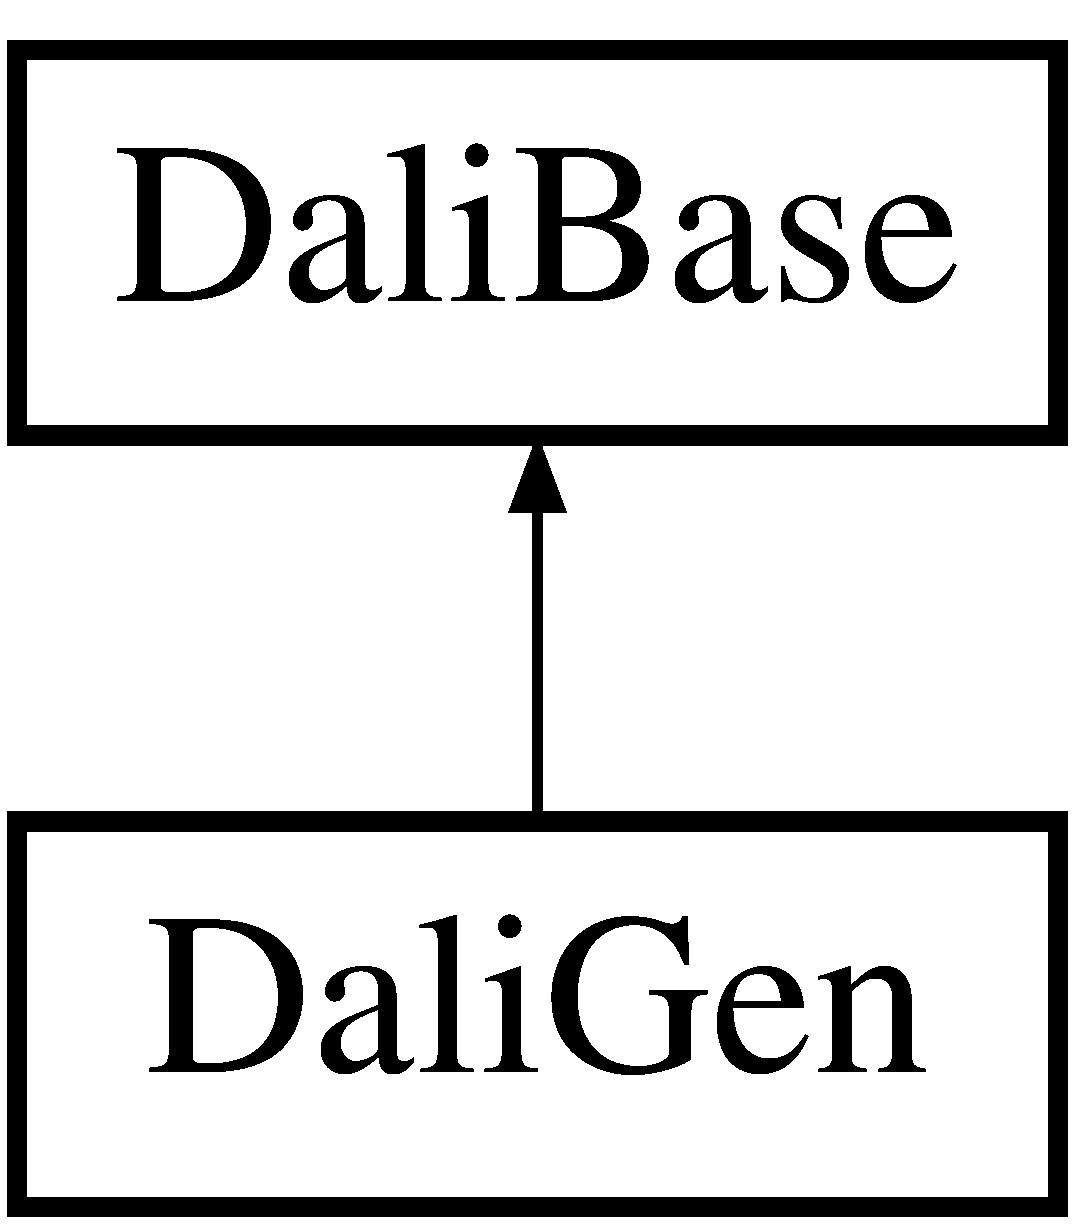
\includegraphics[height=2.000000cm]{classDaliBase}
\end{center}
\end{figure}
\subsection*{Public Types}
\begin{DoxyCompactItemize}
\item 
\hypertarget{classDaliBase_ad587f8c3da29a7e58727872d2a27eeb3}{typedef double(Dali\-Base\-::$\ast$ {\bfseries Mem\-Fun\-Point} )(vector$<$ double $>$ x)}\label{classDaliBase_ad587f8c3da29a7e58727872d2a27eeb3}

\end{DoxyCompactItemize}
\subsection*{Public Member Functions}
\begin{DoxyCompactItemize}
\item 
\hyperlink{classDaliBase_a7ea85e708de3877d9a771d93ea76d617}{Dali\-Base} (int theo, int indep, int noof, vector$<$ double $>$ fidin, string outdir\-\_\-in)
\item 
void \hyperlink{classDaliBase_af6a34db604769e09853e8300dc17fd7c}{Base\-Free} ()
\item 
\hypertarget{classDaliBase_a07d372be1ae30d25a7fd5444042585c4}{double {\bfseries first} (Mem\-Fun\-Point p, vector$<$ double $>$ eval, int par, double step=1e-\/3)}\label{classDaliBase_a07d372be1ae30d25a7fd5444042585c4}

\item 
\hypertarget{classDaliBase_a546624effef5b36ffc555ad13de1709b}{double {\bfseries sec\-One} (Mem\-Fun\-Point p, vector$<$ double $>$ eval, int par, double step=1e-\/2)}\label{classDaliBase_a546624effef5b36ffc555ad13de1709b}

\item 
\hypertarget{classDaliBase_a23a77b29f9d2d66f01327220ed1a9440}{double {\bfseries second} (Mem\-Fun\-Point p, vector$<$ double $>$ eval, int par1, int par2, double step=1e-\/2)}\label{classDaliBase_a23a77b29f9d2d66f01327220ed1a9440}

\item 
\hypertarget{classDaliBase_a1befad16dea2fdbd9e400e7a046f9b3f}{double {\bfseries third} (Mem\-Fun\-Point p, vector$<$ double $>$ eval, int par1, int par2, int par3, double step=1e-\/3)}\label{classDaliBase_a1befad16dea2fdbd9e400e7a046f9b3f}

\item 
virtual double \hyperlink{classDaliBase_ab19c9c960d914f5b8269237420deb8ca}{Phys\-Mod} (vector$<$ double $>$ pars\-\_\-and\-\_\-indep)=0
\item 
virtual double \hyperlink{classDaliBase_af8e98eb7184370d8d64b3b55bc395c6c}{Data\-Cov\-Matrix} (vector$<$ double $>$ pars, int i, int j)=0
\item 
virtual void \hyperlink{classDaliBase_ac0acf75f804718d75ba8ec375c342fad}{Declare\-Data} ()=0
\item 
\hypertarget{classDaliBase_a0c6137241ae1f7c543cd3b6694f5198f}{void {\bfseries Calc\-First\-Dmod} ()}\label{classDaliBase_a0c6137241ae1f7c543cd3b6694f5198f}

\item 
\hypertarget{classDaliBase_aca71df68c84675b37620437721696ef0}{void {\bfseries Calc\-Scnd\-Dmod} ()}\label{classDaliBase_aca71df68c84675b37620437721696ef0}

\item 
\hypertarget{classDaliBase_ac73f100410c08b92e448784bcc5bf6c1}{void {\bfseries Calc\-Thrd\-Dmod} ()}\label{classDaliBase_ac73f100410c08b92e448784bcc5bf6c1}

\item 
void \hyperlink{classDaliBase_aff17417c8d73ab2d75d8f54c7d1ea7d1}{Print\-First\-Dmod} ()
\item 
void \hyperlink{classDaliBase_a9ec7ff196ea59635727ba378b481aa40}{Print\-Scnd\-Dmod} ()
\item 
void \hyperlink{classDaliBase_a55b1ecf5e2f75758ef1aa7c6614bc642}{Print\-Thrd\-Dmod} ()
\item 
void \hyperlink{classDaliBase_a28df9c6ce107f5c8c1e757c2a5924d04}{Plot\-Matrix} (gsl\-\_\-matrix $\ast$To\-Be\-Plotted, int dim, string filesuffix)
\item 
\hypertarget{classDaliBase_add3632260f70ee5286d795f2e7f773d1}{void {\bfseries Fill\-Data\-Cov\-Mat} ()}\label{classDaliBase_add3632260f70ee5286d795f2e7f773d1}

\item 
\hypertarget{classDaliBase_ac63422e32e8fb16a9eda2b8da3a1f944}{void {\bfseries Dali\-Check\-Data\-Decl} ()}\label{classDaliBase_ac63422e32e8fb16a9eda2b8da3a1f944}

\item 
void \hyperlink{classDaliBase_af6ce56b286ef5f014c74ae9f83051e19}{Dali\-Save} (string filesuffix)
\item 
void \hyperlink{classDaliBase_a8cdc64cd3dd46ce4ce1a70f87061dda9}{Parameterdependence} (bool model, bool covmat)
\item 
void \hyperlink{classDaliBase_a8cd32906da8de171eff331ce09d256f2}{Set\-Steps} (double f\-\_\-step, double d\-\_\-step, double t\-\_\-step)
\item 
\hypertarget{classDaliBase_a0f273ab603afac40a8939e20a64feb80}{void {\bfseries Check\-Data\-Size} ()}\label{classDaliBase_a0f273ab603afac40a8939e20a64feb80}

\item 
void \hyperlink{classDaliBase_a75d9801166752bd17af5a30ca24aea20}{Set\-Verbosity} (int v)
\item 
void \hyperlink{classDaliBase_a29c3f9350f4f0990bd803814f4ec7137}{Set\-Diagonal} ()
\item 
void \hyperlink{classDaliBase_a23e24dbbfeadd57d77bfd7921863c744}{Conduct\-Recommended\-Checks} (int a)
\end{DoxyCompactItemize}
\subsection*{Public Attributes}
\begin{DoxyCompactItemize}
\item 
\hypertarget{classDaliBase_a85702051649d311856fe82ea32b1c7f1}{string {\bfseries outdir}}\label{classDaliBase_a85702051649d311856fe82ea32b1c7f1}

\item 
\hypertarget{classDaliBase_a0985d1e2f659e549ca34196015c75cb5}{bool {\bfseries modeldep}}\label{classDaliBase_a0985d1e2f659e549ca34196015c75cb5}

\item 
\hypertarget{classDaliBase_aa968c6982295a041de7106219a3c1ba3}{bool {\bfseries covmatdep}}\label{classDaliBase_aa968c6982295a041de7106219a3c1ba3}

\item 
\hypertarget{classDaliBase_a83a7d058afbf37e695915cb8782b2df3}{bool {\bfseries is\-\_\-diag}}\label{classDaliBase_a83a7d058afbf37e695915cb8782b2df3}

\item 
\hypertarget{classDaliBase_a9dc741756fbf9b438fcef52ba7ae2cd0}{int {\bfseries theodim}}\label{classDaliBase_a9dc741756fbf9b438fcef52ba7ae2cd0}

\item 
\hypertarget{classDaliBase_a191cbbcaaeb7ec14c1fe8bf4f7646e22}{int {\bfseries indepdim}}\label{classDaliBase_a191cbbcaaeb7ec14c1fe8bf4f7646e22}

\item 
int \hyperlink{classDaliBase_abbecb7f25a3040e674377cd9915f1183}{noofdat}
\item 
\hypertarget{classDaliBase_a18d2259363ec995e590a6ae96dee296a}{double {\bfseries fstep}}\label{classDaliBase_a18d2259363ec995e590a6ae96dee296a}

\item 
\hypertarget{classDaliBase_aabcb7e312a672ccc6f294934159f8fe4}{double {\bfseries dstep}}\label{classDaliBase_aabcb7e312a672ccc6f294934159f8fe4}

\item 
\hypertarget{classDaliBase_aa435a0b2ecdc1f9de7dd73705e22d610}{double {\bfseries tstep}}\label{classDaliBase_aa435a0b2ecdc1f9de7dd73705e22d610}

\item 
\hypertarget{classDaliBase_a2730078ea381c17ba37922b1c19ea7ec}{int {\bfseries verbosity}}\label{classDaliBase_a2730078ea381c17ba37922b1c19ea7ec}

\item 
\hypertarget{classDaliBase_aa73ef6f87c8e93d48c64611753eeb936}{int {\bfseries Recommended\-Checks}}\label{classDaliBase_aa73ef6f87c8e93d48c64611753eeb936}

\item 
vector$<$ vector$<$ double $>$ $>$ \hyperlink{classDaliBase_abe548366dfd28590f8db1f681bb1b77d}{datavaribs}
\item 
gsl\-\_\-matrix $\ast$ \hyperlink{classDaliBase_ac287ff97afe28a93bda558357beaee0d}{datapoint\-\_\-weights}
\item 
\hypertarget{classDaliBase_acc9bb2f0566d88a5876675ed3851b0b1}{gsl\-\_\-matrix $\ast$ {\bfseries fisher}}\label{classDaliBase_acc9bb2f0566d88a5876675ed3851b0b1}

\item 
\hypertarget{classDaliBase_a0afc645ad45078e4c3497fe71549a7d9}{vector$<$ vector$<$ vector$<$ double $>$ $>$ $>$ {\bfseries Sabg}}\label{classDaliBase_a0afc645ad45078e4c3497fe71549a7d9}

\item 
\hypertarget{classDaliBase_a431a69681b94c3e25c27726a4aad26e3}{vector$<$ vector$<$ vector$<$ vector\\*
$<$ double $>$ $>$ $>$ $>$ {\bfseries Qabgd}}\label{classDaliBase_a431a69681b94c3e25c27726a4aad26e3}

\item 
\hypertarget{classDaliBase_a0d897fa7e8288582f858ea60f10fae0b}{vector$<$ vector$<$ vector$<$ vector\\*
$<$ vector$<$ double $>$ $>$ $>$ $>$ $>$ {\bfseries Pabgde}}\label{classDaliBase_a0d897fa7e8288582f858ea60f10fae0b}

\item 
\hypertarget{classDaliBase_a2bc46d476c8f956d3c5484a6084e4ee3}{vector$<$ vector$<$ vector$<$ vector\\*
$<$ vector$<$ vector$<$ double $>$ $>$ $>$ $>$ $>$ $>$ {\bfseries Habgdef}}\label{classDaliBase_a2bc46d476c8f956d3c5484a6084e4ee3}

\item 
\hypertarget{classDaliBase_a996d0fec050aec51231beca9c6382875}{vector$<$ vector$<$ vector$<$ int $>$ $>$ $>$ {\bfseries Sabg\-\_\-compute\-\_\-flags}}\label{classDaliBase_a996d0fec050aec51231beca9c6382875}

\item 
\hypertarget{classDaliBase_ae81009c7aa5c2114435908af78cff212}{vector$<$ vector$<$ vector$<$ vector\\*
$<$ int $>$ $>$ $>$ $>$ {\bfseries Qabgd\-\_\-compute\-\_\-flags}}\label{classDaliBase_ae81009c7aa5c2114435908af78cff212}

\item 
\hypertarget{classDaliBase_ae861877710efbfc385397ad6b5deffa4}{vector$<$ vector$<$ vector$<$ vector\\*
$<$ vector$<$ int $>$ $>$ $>$ $>$ $>$ {\bfseries Pabgde\-\_\-compute\-\_\-flags}}\label{classDaliBase_ae861877710efbfc385397ad6b5deffa4}

\item 
\hypertarget{classDaliBase_a020d41ac3e343416350cfbf913c2553d}{vector$<$ vector$<$ vector$<$ vector\\*
$<$ vector$<$ vector$<$ int $>$ $>$ $>$ $>$ $>$ $>$ {\bfseries Habgdef\-\_\-compute\-\_\-flags}}\label{classDaliBase_a020d41ac3e343416350cfbf913c2553d}

\item 
\hypertarget{classDaliBase_a0d7bf539463c26a4dccb73f4c5839a12}{gsl\-\_\-matrix $\ast$ {\bfseries Data\-Cov}}\label{classDaliBase_a0d7bf539463c26a4dccb73f4c5839a12}

\item 
\hypertarget{classDaliBase_a7fd3532925487a8a6d9b5d2b00348b18}{gsl\-\_\-matrix $\ast$ {\bfseries Inv\-Data\-Cov}}\label{classDaliBase_a7fd3532925487a8a6d9b5d2b00348b18}

\item 
bool \hyperlink{classDaliBase_ac19be40e90cba3bdf8fc6a132b3d955d}{datavaribsdeclared}
\item 
\hypertarget{classDaliBase_a10faed76b3954280b83ff927d176acad}{bool {\bfseries checkd}}\label{classDaliBase_a10faed76b3954280b83ff927d176acad}

\item 
\hypertarget{classDaliBase_a3b9da5a51df20cdad2f8b8b7d707eb75}{bool {\bfseries checkdd}}\label{classDaliBase_a3b9da5a51df20cdad2f8b8b7d707eb75}

\item 
\hypertarget{classDaliBase_a6a36213fa6a2f994897540222aee0c41}{bool {\bfseries checkddd}}\label{classDaliBase_a6a36213fa6a2f994897540222aee0c41}

\item 
\hypertarget{classDaliBase_ad4bf365b7b5292a9ee12cceb2c4743a8}{bool {\bfseries covcheck}}\label{classDaliBase_ad4bf365b7b5292a9ee12cceb2c4743a8}

\item 
vector$<$ double $>$ \hyperlink{classDaliBase_ab132077315b2aadc9368a29baec1c8f0}{fid}
\item 
\hypertarget{classDaliBase_a5169cd6353fdccdad05f459ba72efee0}{vector$<$ gsl\-\_\-vector $\ast$ $>$ {\bfseries dmod}}\label{classDaliBase_a5169cd6353fdccdad05f459ba72efee0}

\item 
\hypertarget{classDaliBase_a36bc5d1fe8fc1d592de5b239f60b3359}{vector$<$ vector$<$ gsl\-\_\-vector $\ast$ $>$ $>$ {\bfseries ddmod}}\label{classDaliBase_a36bc5d1fe8fc1d592de5b239f60b3359}

\item 
\hypertarget{classDaliBase_acdd3a0c64d76685c699e05c07c3bc643}{vector$<$ vector$<$ vector\\*
$<$ gsl\-\_\-vector $\ast$ $>$ $>$ $>$ {\bfseries dddmod}}\label{classDaliBase_acdd3a0c64d76685c699e05c07c3bc643}

\end{DoxyCompactItemize}


\subsection{Constructor \& Destructor Documentation}
\hypertarget{classDaliBase_a7ea85e708de3877d9a771d93ea76d617}{\index{Dali\-Base@{Dali\-Base}!Dali\-Base@{Dali\-Base}}
\index{Dali\-Base@{Dali\-Base}!DaliBase@{Dali\-Base}}
\subsubsection[{Dali\-Base}]{\setlength{\rightskip}{0pt plus 5cm}Dali\-Base\-::\-Dali\-Base (
\begin{DoxyParamCaption}
\item[{int}]{theo, }
\item[{int}]{indep, }
\item[{int}]{noof, }
\item[{vector$<$ double $>$}]{fidin, }
\item[{string}]{outdir\-\_\-in}
\end{DoxyParamCaption}
)}}\label{classDaliBase_a7ea85e708de3877d9a771d93ea76d617}
Constructor of the \hyperlink{classDaliBase}{Dali\-Base} class. This constructor is automatically called by the code, and does not need to be acessed by the user. It initializes all the Dali tensors to zero, allocates memory and sets default values for various parameters.
\begin{DoxyItemize}
\item theo\-: the number of theoretical parameters that the user's application depends on
\item indep\-: the number of independent variables that each data point contains. Maybe you have a case where a datapoint is a 3-\/dimensional direction, then you would like to store three coordinates per data point, and consequently you would put indep =3. -\/noof\-: the number of data points, where each data point is considered as one measurement that simultaneously had indep variables under control -\/fidin\-: a vector of length theo. It stores the fiducial values of your theoretical parameters/the maximum likelihood values of your theoretical parameters -\/outdir\-\_\-in\-: specifies the folder in which D\-A\-L\-I will store your results. If the folder does not exist, D\-A\-L\-I creates it 
\end{DoxyItemize}

\subsection{Member Function Documentation}
\hypertarget{classDaliBase_af6a34db604769e09853e8300dc17fd7c}{\index{Dali\-Base@{Dali\-Base}!Base\-Free@{Base\-Free}}
\index{Base\-Free@{Base\-Free}!DaliBase@{Dali\-Base}}
\subsubsection[{Base\-Free}]{\setlength{\rightskip}{0pt plus 5cm}void Dali\-Base\-::\-Base\-Free (
\begin{DoxyParamCaption}
{}
\end{DoxyParamCaption}
)}}\label{classDaliBase_af6a34db604769e09853e8300dc17fd7c}
Deallocates the memory of all pointer-\/like members which D\-A\-L\-I uses \hypertarget{classDaliBase_a23e24dbbfeadd57d77bfd7921863c744}{\index{Dali\-Base@{Dali\-Base}!Conduct\-Recommended\-Checks@{Conduct\-Recommended\-Checks}}
\index{Conduct\-Recommended\-Checks@{Conduct\-Recommended\-Checks}!DaliBase@{Dali\-Base}}
\subsubsection[{Conduct\-Recommended\-Checks}]{\setlength{\rightskip}{0pt plus 5cm}void Dali\-Base\-::\-Conduct\-Recommended\-Checks (
\begin{DoxyParamCaption}
\item[{int}]{a}
\end{DoxyParamCaption}
)}}\label{classDaliBase_a23e24dbbfeadd57d77bfd7921863c744}
If a is greater than zero, the code will produce output files of the derivatives that the user has to check himself. \hypertarget{classDaliBase_af6ce56b286ef5f014c74ae9f83051e19}{\index{Dali\-Base@{Dali\-Base}!Dali\-Save@{Dali\-Save}}
\index{Dali\-Save@{Dali\-Save}!DaliBase@{Dali\-Base}}
\subsubsection[{Dali\-Save}]{\setlength{\rightskip}{0pt plus 5cm}void Dali\-Base\-::\-Dali\-Save (
\begin{DoxyParamCaption}
\item[{string}]{filesuffix}
\end{DoxyParamCaption}
)}}\label{classDaliBase_af6ce56b286ef5f014c74ae9f83051e19}
Saves the Fisher matrix and the Dali tensors to separate files in the outdir. The formatting of the files is \char`\"{}index index index Sabg\-\_\-\-Tensor entry\char`\"{} in case of the Sabg-\/tensor. For the Fisher matrix and the higher order tensors the same formatting is chosen, just with more or less indices, separated by spaces. Keep in mind which index number refers to which parameter. A common question is\-: \char`\"{}\-Why are these tensors not invariant under all permutations
  of the indices? Why is my Sabg\mbox{[}0\mbox{]}\mbox{[}0\mbox{]}\mbox{[}1\mbox{]} not the same as my Sabg\mbox{[}0\mbox{]}\mbox{[}1\mbox{]}\mbox{[}0\mbox{]}?\char`\"{} The reason is that the tensors here used are those of Eq.(14) in arxiv 1401.\-6892\-\_\-v2. -\/filesuffix\-: you may provide some suffix in order to identify the files. \hypertarget{classDaliBase_af8e98eb7184370d8d64b3b55bc395c6c}{\index{Dali\-Base@{Dali\-Base}!Data\-Cov\-Matrix@{Data\-Cov\-Matrix}}
\index{Data\-Cov\-Matrix@{Data\-Cov\-Matrix}!DaliBase@{Dali\-Base}}
\subsubsection[{Data\-Cov\-Matrix}]{\setlength{\rightskip}{0pt plus 5cm}virtual double Dali\-Base\-::\-Data\-Cov\-Matrix (
\begin{DoxyParamCaption}
\item[{vector$<$ double $>$}]{pars, }
\item[{int}]{i, }
\item[{int}]{j}
\end{DoxyParamCaption}
)\hspace{0.3cm}{\ttfamily [pure virtual]}}}\label{classDaliBase_af8e98eb7184370d8d64b3b55bc395c6c}
A pure virtual function that must be overwritten by the user. See the Tutorial on how to achieve this.
\begin{DoxyItemize}
\item pars\-: is a vector of length theodim that holds the theoretical parameters.
\item i and j\-: the entries/elements of the data covariance matrix. If your data covariance matrix depends on the data point datavaribs\mbox{[}i\mbox{]}\mbox{[}j\mbox{]}, use i and j to access datavaribs\mbox{[}i\mbox{]}\mbox{[}j\mbox{]}. The function shall return the (i,j)-\/element of the Data covariance matrix. 
\end{DoxyItemize}\hypertarget{classDaliBase_ac0acf75f804718d75ba8ec375c342fad}{\index{Dali\-Base@{Dali\-Base}!Declare\-Data@{Declare\-Data}}
\index{Declare\-Data@{Declare\-Data}!DaliBase@{Dali\-Base}}
\subsubsection[{Declare\-Data}]{\setlength{\rightskip}{0pt plus 5cm}virtual void Dali\-Base\-::\-Declare\-Data (
\begin{DoxyParamCaption}
{}
\end{DoxyParamCaption}
)\hspace{0.3cm}{\ttfamily [pure virtual]}}}\label{classDaliBase_ac0acf75f804718d75ba8ec375c342fad}
A pure virtual function that must be overwritten by the user. The function must set the datavaribs\mbox{[}i\mbox{]}\mbox{[}j\mbox{]}, where i runs in \mbox{[}0,noofdat-\/1\mbox{]} and j runs in \mbox{[}0,indep-\/1\mbox{]}. At constant i, datavaribs contains the complete ith measurement. The jth independent variable of the ith measurement is then datavaribs\mbox{[}i\mbox{]}\mbox{[}j\mbox{]}. The function must end with \char`\"{}datavaribsdeclared=1;\char`\"{} This tells the code that it now knows the independent variables. \hypertarget{classDaliBase_a8cdc64cd3dd46ce4ce1a70f87061dda9}{\index{Dali\-Base@{Dali\-Base}!Parameterdependence@{Parameterdependence}}
\index{Parameterdependence@{Parameterdependence}!DaliBase@{Dali\-Base}}
\subsubsection[{Parameterdependence}]{\setlength{\rightskip}{0pt plus 5cm}void Dali\-Base\-::\-Parameterdependence (
\begin{DoxyParamCaption}
\item[{bool}]{model, }
\item[{bool}]{covmat}
\end{DoxyParamCaption}
)}}\label{classDaliBase_a8cdc64cd3dd46ce4ce1a70f87061dda9}
Telling D\-A\-L\-I whether the model and/or the covariance matrix are parameter dependend. If model == 0, then the model is treated as parameter indepenend, if covmat == 0, then the covariance matrix is treated as independend, and no derivatives of the corresponding quantities will be calculated. This speeds up D\-A\-L\-I. \hypertarget{classDaliBase_ab19c9c960d914f5b8269237420deb8ca}{\index{Dali\-Base@{Dali\-Base}!Phys\-Mod@{Phys\-Mod}}
\index{Phys\-Mod@{Phys\-Mod}!DaliBase@{Dali\-Base}}
\subsubsection[{Phys\-Mod}]{\setlength{\rightskip}{0pt plus 5cm}virtual double Dali\-Base\-::\-Phys\-Mod (
\begin{DoxyParamCaption}
\item[{vector$<$ double $>$}]{pars\-\_\-and\-\_\-indep}
\end{DoxyParamCaption}
)\hspace{0.3cm}{\ttfamily [pure virtual]}}}\label{classDaliBase_ab19c9c960d914f5b8269237420deb8ca}
A pure virtual function that must be overwritten by the user. The vector pars\-\_\-and\-\_\-indep has length theodim+indep. Its first theodim entries are reserved for the parameters, its last indep entries are reserved for independent variables. The function shall return the modelprediction as a function of the theoretical parameters and the independent variables. The ordering is important\-: The code will only take derivatives of this function with respect to its first theodim parameters. \hypertarget{classDaliBase_a28df9c6ce107f5c8c1e757c2a5924d04}{\index{Dali\-Base@{Dali\-Base}!Plot\-Matrix@{Plot\-Matrix}}
\index{Plot\-Matrix@{Plot\-Matrix}!DaliBase@{Dali\-Base}}
\subsubsection[{Plot\-Matrix}]{\setlength{\rightskip}{0pt plus 5cm}void Dali\-Base\-::\-Plot\-Matrix (
\begin{DoxyParamCaption}
\item[{gsl\-\_\-matrix $\ast$}]{To\-Be\-Plotted, }
\item[{int}]{dim, }
\item[{string}]{filesuffix}
\end{DoxyParamCaption}
)}}\label{classDaliBase_a28df9c6ce107f5c8c1e757c2a5924d04}
Creates a file that allows to plot a square matrix. This can be used in order to check whether the derivatives of the covariance matrix seem okay. \hypertarget{classDaliBase_aff17417c8d73ab2d75d8f54c7d1ea7d1}{\index{Dali\-Base@{Dali\-Base}!Print\-First\-Dmod@{Print\-First\-Dmod}}
\index{Print\-First\-Dmod@{Print\-First\-Dmod}!DaliBase@{Dali\-Base}}
\subsubsection[{Print\-First\-Dmod}]{\setlength{\rightskip}{0pt plus 5cm}void Dali\-Base\-::\-Print\-First\-Dmod (
\begin{DoxyParamCaption}
{}
\end{DoxyParamCaption}
)}}\label{classDaliBase_aff17417c8d73ab2d75d8f54c7d1ea7d1}
Prints the first derivatives of the model to a file. Plotting them allows to check whether the finite difference has been adjusted appropriately. \hypertarget{classDaliBase_a9ec7ff196ea59635727ba378b481aa40}{\index{Dali\-Base@{Dali\-Base}!Print\-Scnd\-Dmod@{Print\-Scnd\-Dmod}}
\index{Print\-Scnd\-Dmod@{Print\-Scnd\-Dmod}!DaliBase@{Dali\-Base}}
\subsubsection[{Print\-Scnd\-Dmod}]{\setlength{\rightskip}{0pt plus 5cm}void Dali\-Base\-::\-Print\-Scnd\-Dmod (
\begin{DoxyParamCaption}
{}
\end{DoxyParamCaption}
)}}\label{classDaliBase_a9ec7ff196ea59635727ba378b481aa40}
Writes the second derivatives of the model to the file outdir/\-Second\-Derivs \hypertarget{classDaliBase_a55b1ecf5e2f75758ef1aa7c6614bc642}{\index{Dali\-Base@{Dali\-Base}!Print\-Thrd\-Dmod@{Print\-Thrd\-Dmod}}
\index{Print\-Thrd\-Dmod@{Print\-Thrd\-Dmod}!DaliBase@{Dali\-Base}}
\subsubsection[{Print\-Thrd\-Dmod}]{\setlength{\rightskip}{0pt plus 5cm}void Dali\-Base\-::\-Print\-Thrd\-Dmod (
\begin{DoxyParamCaption}
{}
\end{DoxyParamCaption}
)}}\label{classDaliBase_a55b1ecf5e2f75758ef1aa7c6614bc642}
Writes the third derivatives of the model to the file outdir/\-Third\-Derivs \hypertarget{classDaliBase_a29c3f9350f4f0990bd803814f4ec7137}{\index{Dali\-Base@{Dali\-Base}!Set\-Diagonal@{Set\-Diagonal}}
\index{Set\-Diagonal@{Set\-Diagonal}!DaliBase@{Dali\-Base}}
\subsubsection[{Set\-Diagonal}]{\setlength{\rightskip}{0pt plus 5cm}void Dali\-Base\-::\-Set\-Diagonal (
\begin{DoxyParamCaption}
{}
\end{DoxyParamCaption}
)}}\label{classDaliBase_a29c3f9350f4f0990bd803814f4ec7137}
If the data covariance matrix is diagonal, the user can call this member function to speed up the execution of the code. \hypertarget{classDaliBase_a8cd32906da8de171eff331ce09d256f2}{\index{Dali\-Base@{Dali\-Base}!Set\-Steps@{Set\-Steps}}
\index{Set\-Steps@{Set\-Steps}!DaliBase@{Dali\-Base}}
\subsubsection[{Set\-Steps}]{\setlength{\rightskip}{0pt plus 5cm}void Dali\-Base\-::\-Set\-Steps (
\begin{DoxyParamCaption}
\item[{double}]{f\-\_\-step, }
\item[{double}]{d\-\_\-step, }
\item[{double}]{t\-\_\-step}
\end{DoxyParamCaption}
)}}\label{classDaliBase_a8cd32906da8de171eff331ce09d256f2}
Allows the user to change the finite difference steps, that are used for the numerical evaluation of the derivatives for the M\-O\-D\-E\-L. A corresponding function exists for the finite difference steps for the covariance matrix. -\/f\-\_\-step\-: the finite difference step for the first derivatives of the model -\/d\-\_\-step\-: for the second derivatives of the model -\/t\-\_\-step\-: for the thrid derivatives of the model \hypertarget{classDaliBase_a75d9801166752bd17af5a30ca24aea20}{\index{Dali\-Base@{Dali\-Base}!Set\-Verbosity@{Set\-Verbosity}}
\index{Set\-Verbosity@{Set\-Verbosity}!DaliBase@{Dali\-Base}}
\subsubsection[{Set\-Verbosity}]{\setlength{\rightskip}{0pt plus 5cm}void Dali\-Base\-::\-Set\-Verbosity (
\begin{DoxyParamCaption}
\item[{int}]{v}
\end{DoxyParamCaption}
)}}\label{classDaliBase_a75d9801166752bd17af5a30ca24aea20}
If v $>$ 1, the code will print more messages to the screen. 

\subsection{Member Data Documentation}
\hypertarget{classDaliBase_ac287ff97afe28a93bda558357beaee0d}{\index{Dali\-Base@{Dali\-Base}!datapoint\-\_\-weights@{datapoint\-\_\-weights}}
\index{datapoint\-\_\-weights@{datapoint\-\_\-weights}!DaliBase@{Dali\-Base}}
\subsubsection[{datapoint\-\_\-weights}]{\setlength{\rightskip}{0pt plus 5cm}gsl\-\_\-matrix$\ast$ Dali\-Base\-::datapoint\-\_\-weights}}\label{classDaliBase_ac287ff97afe28a93bda558357beaee0d}
A gsl\-\_\-matrix$\ast$ that allows you to multiply data points with a weight. The weights must be constant; i.\-e. they cannot depend on parameters. Abbreviating the datapoint\-\_\-weights matrix by W, the loglikelihood is given by L = -\/1/2 ( (\{d\} -\/ \{m\}) W C$^\wedge$\{-\/1\} (\{d\} -\/ \{m\} ) ). \hypertarget{classDaliBase_abe548366dfd28590f8db1f681bb1b77d}{\index{Dali\-Base@{Dali\-Base}!datavaribs@{datavaribs}}
\index{datavaribs@{datavaribs}!DaliBase@{Dali\-Base}}
\subsubsection[{datavaribs}]{\setlength{\rightskip}{0pt plus 5cm}vector$<$vector$<$ double $>$ $>$ Dali\-Base\-::datavaribs}}\label{classDaliBase_abe548366dfd28590f8db1f681bb1b77d}
$\ast$\-Storage room for the data. The structure $<$vector$<$vector$<$double $>$ $>$ works like a C-\/array ar\mbox{[}i\mbox{]}\mbox{[}j\mbox{]}, and is also called like this\-: datavaribs\mbox{[}i\mbox{]}\mbox{[}j\mbox{]} is the jth independent variable if the ith datapoint. I.\-e. each datavaribs\mbox{[}i\mbox{]}\mbox{[}j\mbox{]} is of type double. Each datavaribs\mbox{[}i\mbox{]} is a vector of doubles. Each of the vectors datavaribs\mbox{[}i\mbox{]} will later be inserted into the Phys\-Mod, as a point where derivatives are taken. Make sure to correctly distribute your data into this array. If you have 50 data points, the index i of datavaribs\mbox{[}i\mbox{]}\mbox{[}j\mbox{]} will run from 0 to 49. If you have only one independent variable, only datavaribs\mbox{[}i\mbox{]}\mbox{[}0\mbox{]} will exist. So a cosmologist could for example set datavaribs\mbox{[}i\mbox{]}\mbox{[}0\mbox{]} = redshift\mbox{[}i\mbox{]}. The code resizes datavaribs for you\-: it will have dimensions noofdat (the number of datapoints) times indep (the number of independent variables). Do not resize this vector to your convenience! Also don't use push\-\_\-back(). \hypertarget{classDaliBase_ac19be40e90cba3bdf8fc6a132b3d955d}{\index{Dali\-Base@{Dali\-Base}!datavaribsdeclared@{datavaribsdeclared}}
\index{datavaribsdeclared@{datavaribsdeclared}!DaliBase@{Dali\-Base}}
\subsubsection[{datavaribsdeclared}]{\setlength{\rightskip}{0pt plus 5cm}bool Dali\-Base\-::datavaribsdeclared}}\label{classDaliBase_ac19be40e90cba3bdf8fc6a132b3d955d}
A flag that must be set by the function \hyperlink{classDaliBase_ac0acf75f804718d75ba8ec375c342fad}{Declare\-Data()}, after the user has stored the data in the vector datavaribs \hypertarget{classDaliBase_ab132077315b2aadc9368a29baec1c8f0}{\index{Dali\-Base@{Dali\-Base}!fid@{fid}}
\index{fid@{fid}!DaliBase@{Dali\-Base}}
\subsubsection[{fid}]{\setlength{\rightskip}{0pt plus 5cm}vector$<$double$>$ Dali\-Base\-::fid}}\label{classDaliBase_ab132077315b2aadc9368a29baec1c8f0}
Stores the values of the parameters at the maximum likelihood point (for forecasting, this is also called 'the fiducial'. At this point, D\-A\-L\-I will evaluate the derivatives. The resulting D\-A\-L\-I-\/tensors will depend on the choice of the fiducial point! If you change the fiducial, you will have to recalculate your tensors. \hypertarget{classDaliBase_abbecb7f25a3040e674377cd9915f1183}{\index{Dali\-Base@{Dali\-Base}!noofdat@{noofdat}}
\index{noofdat@{noofdat}!DaliBase@{Dali\-Base}}
\subsubsection[{noofdat}]{\setlength{\rightskip}{0pt plus 5cm}int Dali\-Base\-::noofdat}}\label{classDaliBase_abbecb7f25a3040e674377cd9915f1183}
The number of data points. 

The documentation for this class was generated from the following files\-:\begin{DoxyCompactItemize}
\item 
Dali\-Base.\-h\item 
Dali\-Base.\-cpp\end{DoxyCompactItemize}

\hypertarget{classDaliGen}{\section{Dali\-Gen Class Reference}
\label{classDaliGen}\index{Dali\-Gen@{Dali\-Gen}}
}
Inheritance diagram for Dali\-Gen\-:\begin{figure}[H]
\begin{center}
\leavevmode
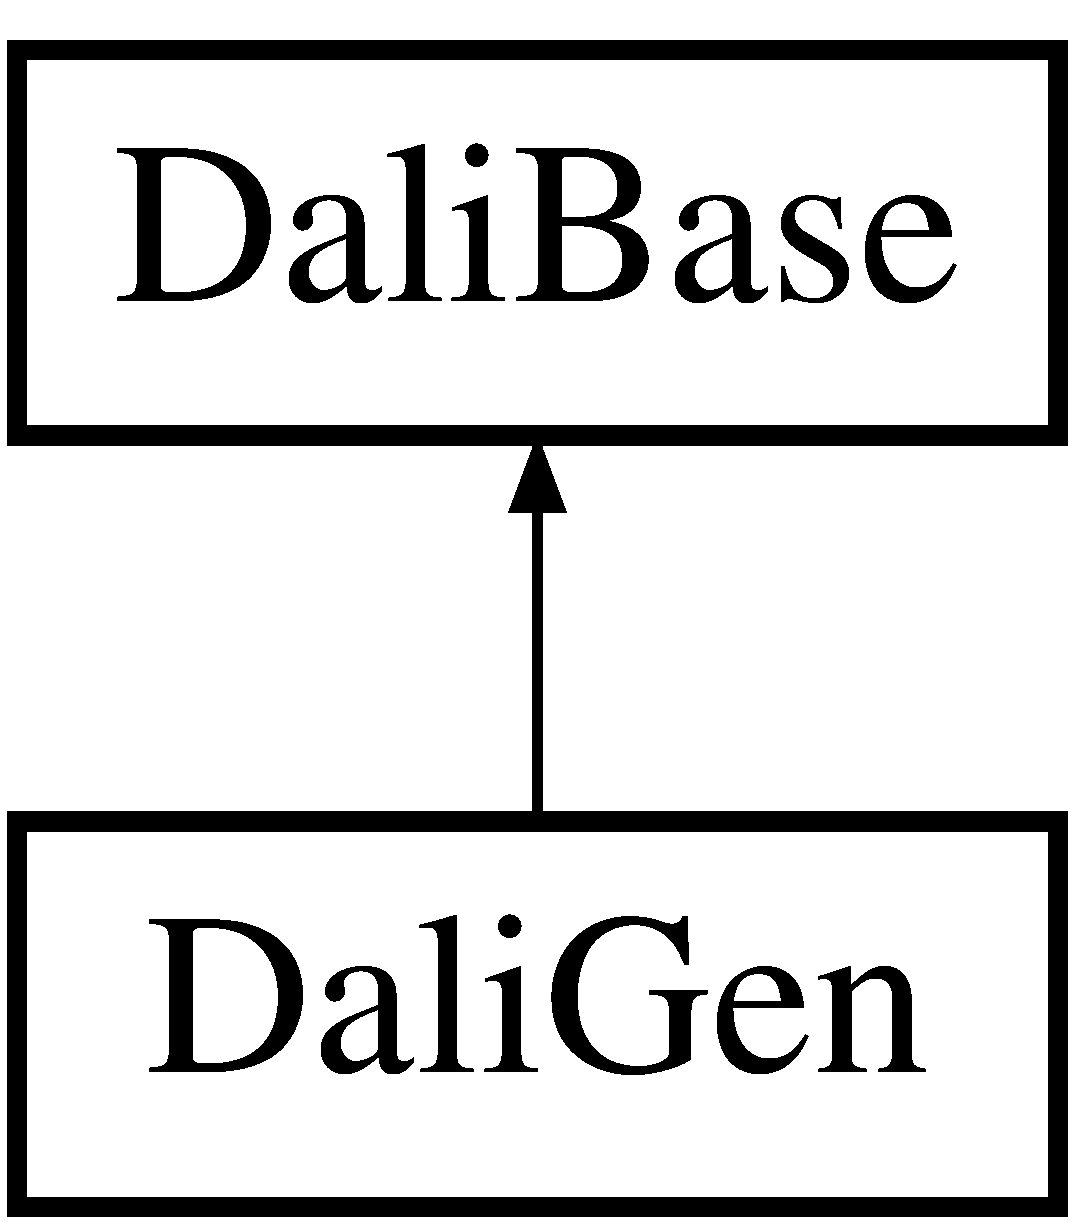
\includegraphics[height=2.000000cm]{classDaliGen}
\end{center}
\end{figure}
\subsection*{Public Types}
\begin{DoxyCompactItemize}
\item 
\hypertarget{classDaliGen_a2c740d6c4e6022d602757a84a41784cd}{typedef double(Dali\-Gen\-::$\ast$ {\bfseries matrixfiller} )(vector$<$ double $>$ eval, int i, int j)}\label{classDaliGen_a2c740d6c4e6022d602757a84a41784cd}

\end{DoxyCompactItemize}
\subsection*{Public Member Functions}
\begin{DoxyCompactItemize}
\item 
\hyperlink{classDaliGen_a0bba3e7de4d7362c28047cf7f4cb41ec}{Dali\-Gen} (int theo, int indep, int noof, vector$<$ double $>$ fidin, int derivorder\-\_\-in, string outdir\-\_\-in)
\item 
\hypertarget{classDaliGen_adc1822fa12310cc961f616b9a861963e}{double {\bfseries sec\-One\-Mat} (matrixfiller p, vector$<$ double $>$ eval, int par, int i, int j, double step=2e-\/2)}\label{classDaliGen_adc1822fa12310cc961f616b9a861963e}

\item 
\hypertarget{classDaliGen_a66103dcbc54e36a98f4fdc39bb206f5a}{void {\bfseries D\-Matrix} (matrixfiller p, vector$<$ double $>$ eval, int par, int matrixdim, gsl\-\_\-matrix $\ast$result, double step=0.\-01)}\label{classDaliGen_a66103dcbc54e36a98f4fdc39bb206f5a}

\item 
\hypertarget{classDaliGen_a34beadec0b421cfaaeb37f9fc92a730d}{double {\bfseries sec\-One\-Mat} (matrixfiller p, vector$<$ double $>$ eval, int par, int matrixdim, gsl\-\_\-matrix $\ast$result, double step=0.\-01)}\label{classDaliGen_a34beadec0b421cfaaeb37f9fc92a730d}

\item 
\hypertarget{classDaliGen_a6ff2c1a3cdd2a953c6207f04b5379646}{void {\bfseries D\-D\-Matrix} (matrixfiller p, vector$<$ double $>$ eval, int par1, int par2, int matrixdim, gsl\-\_\-matrix $\ast$result, double step=0.\-01)}\label{classDaliGen_a6ff2c1a3cdd2a953c6207f04b5379646}

\item 
\hypertarget{classDaliGen_a63b4d29fc5c02ef5cad74e96c318cdf2}{void {\bfseries D\-D\-D\-Matrix} (matrixfiller p, vector$<$ double $>$ eval, int par1, int par2, int par3, int matrixdim, gsl\-\_\-matrix $\ast$result, double step=0.\-01)}\label{classDaliGen_a63b4d29fc5c02ef5cad74e96c318cdf2}

\item 
void \hyperlink{classDaliGen_a9ad9ceddbb0b7d156c7eeeda08a0fc32}{Set\-Steps\-\_\-\-Cov} (double f\-\_\-step\-\_\-\-C, double d\-\_\-step\-\_\-\-C, double t\-\_\-step\-\_\-\-C)
\item 
\hypertarget{classDaliGen_ae4ac3d0ff453bc1e8dc7932284f1e745}{void {\bfseries Calc\-\_\-\-D\-Cs} ()}\label{classDaliGen_ae4ac3d0ff453bc1e8dc7932284f1e745}

\item 
\hypertarget{classDaliGen_ae72c88dd2c32b17f052423e97cfddf12}{void {\bfseries Calc\-\_\-\-D\-D\-Cs} ()}\label{classDaliGen_ae72c88dd2c32b17f052423e97cfddf12}

\item 
\hypertarget{classDaliGen_a50fe1b2e0aa35d09b8c4e4b9481afc41}{void {\bfseries Calc\-\_\-\-D\-D\-D\-Cs} ()}\label{classDaliGen_a50fe1b2e0aa35d09b8c4e4b9481afc41}

\item 
\hypertarget{classDaliGen_a2560914669d9b8d6dce111e15de84e9b}{void {\bfseries Fill\-Ctwiddle} ()}\label{classDaliGen_a2560914669d9b8d6dce111e15de84e9b}

\item 
\hypertarget{classDaliGen_af8e6bab9599a2f69cfdcfd1fe7e56c9c}{void {\bfseries Double\-Twiddle} ()}\label{classDaliGen_af8e6bab9599a2f69cfdcfd1fe7e56c9c}

\item 
void \hyperlink{classDaliGen_a43f374299add9948a7853c7d0427cbe9}{Calc\-Fisher} ()
\item 
void \hyperlink{classDaliGen_ace06507c0cf05995ea4b07fddc195835}{Calc\-\_\-\-Beyond\-Fish} ()
\item 
void \hyperlink{classDaliGen_a598555d704eb5387c11e26e0785637c7}{Free} ()
\item 
void \hyperlink{classDaliGen_a4b3d983bea7db5c7ba634fd3e96864ed}{Low\-Memory} ()
\end{DoxyCompactItemize}
\subsection*{Public Attributes}
\begin{DoxyCompactItemize}
\item 
\hypertarget{classDaliGen_a69f098a299de5d0d018cf8edcdd2d4d2}{vector$<$ gsl\-\_\-matrix $\ast$ $>$ {\bfseries D\-Cov}}\label{classDaliGen_a69f098a299de5d0d018cf8edcdd2d4d2}

\item 
\hypertarget{classDaliGen_af205ad401e1df65def06d7d0f0b149e9}{vector$<$ vector$<$ gsl\-\_\-matrix $\ast$ $>$ $>$ {\bfseries D\-D\-Cov}}\label{classDaliGen_af205ad401e1df65def06d7d0f0b149e9}

\item 
\hypertarget{classDaliGen_aa4df079f30dc2365ca1c197bb32f46e7}{vector$<$ vector$<$ vector\\*
$<$ gsl\-\_\-matrix $\ast$ $>$ $>$ $>$ {\bfseries D\-D\-D\-Cov}}\label{classDaliGen_aa4df079f30dc2365ca1c197bb32f46e7}

\item 
\hypertarget{classDaliGen_a69bb99704cd878a9309adee522466e78}{vector$<$ gsl\-\_\-matrix $\ast$ $>$ {\bfseries Ctwiddle}}\label{classDaliGen_a69bb99704cd878a9309adee522466e78}

\item 
\hypertarget{classDaliGen_acbaa76829d7cf685291b1e67579883f2}{vector$<$ vector$<$ gsl\-\_\-matrix $\ast$ $>$ $>$ {\bfseries C\-Doubletwiddle}}\label{classDaliGen_acbaa76829d7cf685291b1e67579883f2}

\item 
\hypertarget{classDaliGen_abdff7f7f88cb0f00127e11e1b2ec9ba7}{vector$<$ vector$<$ vector\\*
$<$ gsl\-\_\-matrix $\ast$ $>$ $>$ $>$ {\bfseries C\-Tripletwiddle}}\label{classDaliGen_abdff7f7f88cb0f00127e11e1b2ec9ba7}

\end{DoxyCompactItemize}


\subsection{Constructor \& Destructor Documentation}
\hypertarget{classDaliGen_a0bba3e7de4d7362c28047cf7f4cb41ec}{\index{Dali\-Gen@{Dali\-Gen}!Dali\-Gen@{Dali\-Gen}}
\index{Dali\-Gen@{Dali\-Gen}!DaliGen@{Dali\-Gen}}
\subsubsection[{Dali\-Gen}]{\setlength{\rightskip}{0pt plus 5cm}Dali\-Gen\-::\-Dali\-Gen (
\begin{DoxyParamCaption}
\item[{int}]{theo, }
\item[{int}]{indep, }
\item[{int}]{noof, }
\item[{vector$<$ double $>$}]{fidin, }
\item[{int}]{derivorder\-\_\-in, }
\item[{string}]{outdir\-\_\-in}
\end{DoxyParamCaption}
)}}\label{classDaliGen_a0bba3e7de4d7362c28047cf7f4cb41ec}
Constructor of a general dali object. The vectors which hold your parameters, the covariance matrix and its derivatives are allocated. Boolean flags are set to zero, indicating that nothing has been calculated yet. This constructor needs to be given the following parameters\-:
\begin{DoxyItemize}
\item int theo\-: the number of theoretical parameters, i.\-e. the dimensionality of your likelihood in parameter space
\item int indep\-: the number of independent variables, that your data depend on. So basically everything that is not a theoretical parameter but still goes into the data. In cosmology this could be e.\-g. the redshift or the mass of some object. indep can be larger than 1, if your data depend on more than one independent variable, for example on time A\-N\-D temperature, as in case of the fishes that are described in the manual.
\item int noof\-: the number of data points in your data set
\item vector $<$double$>$ fidin\-: a vector of length theo, that contains the values of your fiducial parameters. The order of the parameters must be kept the same throughout the code! So please remember which parameter you store at position fidin\mbox{[}i\mbox{]}.
\item int derivorder\-: if set to one D\-A\-L\-I will calculate third derivatives, if zero, D\-A\-L\-I will stop at second order derivatives
\item string outdir\-\_\-in\-: tells the code where to store its results. If the folder outdir\-\_\-in does not exist, D\-A\-L\-I will create it. If it exists, it will not be overwritten. 
\end{DoxyItemize}

\subsection{Member Function Documentation}
\hypertarget{classDaliGen_ace06507c0cf05995ea4b07fddc195835}{\index{Dali\-Gen@{Dali\-Gen}!Calc\-\_\-\-Beyond\-Fish@{Calc\-\_\-\-Beyond\-Fish}}
\index{Calc\-\_\-\-Beyond\-Fish@{Calc\-\_\-\-Beyond\-Fish}!DaliGen@{Dali\-Gen}}
\subsubsection[{Calc\-\_\-\-Beyond\-Fish}]{\setlength{\rightskip}{0pt plus 5cm}void Dali\-Gen\-::\-Calc\-\_\-\-Beyond\-Fish (
\begin{DoxyParamCaption}
{}
\end{DoxyParamCaption}
)}}\label{classDaliGen_ace06507c0cf05995ea4b07fddc195835}
Calculates the higher order Dali-\/\-Tensors that approximate the likelihood beyond what the fisher matrix can do. It checks whether everything has been calculated that is needed. If not, it will do so. The resulting Dali tensors are stored in Dali\-Gen\-\_\-object.\-Sabg, Dali\-Gen\-\_\-object.\-Qabgd, Dali\-Gen\-\_\-object.\-Pabgde, Dali\-Gen\-\_\-object.\-Habgdef, where Dali\-Gen\-\_\-object is the name of the object that you created in your main() A\-T\-T\-E\-N\-T\-I\-O\-N\-: depending on whether you requested second or third order derivatives for your model and/or your likelihood, the tensor Qabgd will change, depending on the number of derivatives. \hypertarget{classDaliGen_a43f374299add9948a7853c7d0427cbe9}{\index{Dali\-Gen@{Dali\-Gen}!Calc\-Fisher@{Calc\-Fisher}}
\index{Calc\-Fisher@{Calc\-Fisher}!DaliGen@{Dali\-Gen}}
\subsubsection[{Calc\-Fisher}]{\setlength{\rightskip}{0pt plus 5cm}void Dali\-Gen\-::\-Calc\-Fisher (
\begin{DoxyParamCaption}
{}
\end{DoxyParamCaption}
)}}\label{classDaliGen_a43f374299add9948a7853c7d0427cbe9}
Calculates the Fisher matrix and stores it in the gsl\-\_\-matrix$\ast$ Dali\-Gen\-\_\-object.\-fisher . The code will automatically check whether everything has been computed that it needs for the fisher matrix. If not, it will do so. If the Fisher matrix is singular, it doesn't matter much for the D\-A\-L\-I contours of the likelihood. The code will however warn you that you shall not use the fisher matrix as a proposal distribution for the M\-C\-M\-C sampler. \hypertarget{classDaliGen_a598555d704eb5387c11e26e0785637c7}{\index{Dali\-Gen@{Dali\-Gen}!Free@{Free}}
\index{Free@{Free}!DaliGen@{Dali\-Gen}}
\subsubsection[{Free}]{\setlength{\rightskip}{0pt plus 5cm}void Dali\-Gen\-::\-Free (
\begin{DoxyParamCaption}
{}
\end{DoxyParamCaption}
)}}\label{classDaliGen_a598555d704eb5387c11e26e0785637c7}
Frees the memory associated with the pointers in the \hyperlink{classDaliGen}{Dali\-Gen} class. \hypertarget{classDaliGen_a4b3d983bea7db5c7ba634fd3e96864ed}{\index{Dali\-Gen@{Dali\-Gen}!Low\-Memory@{Low\-Memory}}
\index{Low\-Memory@{Low\-Memory}!DaliGen@{Dali\-Gen}}
\subsubsection[{Low\-Memory}]{\setlength{\rightskip}{0pt plus 5cm}void Dali\-Gen\-::\-Low\-Memory (
\begin{DoxyParamCaption}
{}
\end{DoxyParamCaption}
)}}\label{classDaliGen_a4b3d983bea7db5c7ba634fd3e96864ed}
If this function is called before the Dali\-Tensors are calculated, then the code will not keep the derivatives of the covariance matrix in memory. The derivative matrices then cannot be plotted. The Dali\-Tensors can still be calculated (because the code uses the Ctwiddles for that.) \hypertarget{classDaliGen_a9ad9ceddbb0b7d156c7eeeda08a0fc32}{\index{Dali\-Gen@{Dali\-Gen}!Set\-Steps\-\_\-\-Cov@{Set\-Steps\-\_\-\-Cov}}
\index{Set\-Steps\-\_\-\-Cov@{Set\-Steps\-\_\-\-Cov}!DaliGen@{Dali\-Gen}}
\subsubsection[{Set\-Steps\-\_\-\-Cov}]{\setlength{\rightskip}{0pt plus 5cm}void Dali\-Gen\-::\-Set\-Steps\-\_\-\-Cov (
\begin{DoxyParamCaption}
\item[{double}]{f\-\_\-step\-\_\-\-C, }
\item[{double}]{d\-\_\-step\-\_\-\-C, }
\item[{double}]{t\-\_\-step\-\_\-\-C}
\end{DoxyParamCaption}
)}}\label{classDaliGen_a9ad9ceddbb0b7d156c7eeeda08a0fc32}
Allows the user to set the step widths of the finite difference steps when taking derivatives of the covariance matrix. A similar function exists for the derivatives of the physical model. 

The documentation for this class was generated from the following files\-:\begin{DoxyCompactItemize}
\item 
Dali\-Gen.\-h\item 
Dali\-Gen.\-cpp\end{DoxyCompactItemize}

\hypertarget{classDaliPaint}{\section{Dali\-Paint Class Reference}
\label{classDaliPaint}\index{Dali\-Paint@{Dali\-Paint}}
}
\subsection*{Public Types}
\begin{DoxyCompactItemize}
\item 
\hypertarget{classDaliPaint_ac11f93a8b8fef1b6297b6ae0f8773a7e}{typedef vector$<$ vector$<$ vector\\*
$<$ double $>$ $>$ $>$ {\bfseries flex}}\label{classDaliPaint_ac11f93a8b8fef1b6297b6ae0f8773a7e}

\item 
\hypertarget{classDaliPaint_a41852dac3b5c43992a37156bd4003dc8}{typedef vector$<$ vector$<$ vector\\*
$<$ vector$<$ double $>$ $>$ $>$ $>$ {\bfseries quarx}}\label{classDaliPaint_a41852dac3b5c43992a37156bd4003dc8}

\item 
\hypertarget{classDaliPaint_a4223372000c10516d596b2711c8f6e34}{typedef vector$<$ vector$<$ vector\\*
$<$ vector$<$ vector$<$ double $>$ $>$ $>$ $>$ $>$ {\bfseries pent}}\label{classDaliPaint_a4223372000c10516d596b2711c8f6e34}

\item 
\hypertarget{classDaliPaint_a9ec046b9290d513125a98b3029c19137}{typedef vector$<$ vector$<$ vector\\*
$<$ vector$<$ vector$<$ vector\\*
$<$ double $>$ $>$ $>$ $>$ $>$ $>$ {\bfseries hex}}\label{classDaliPaint_a9ec046b9290d513125a98b3029c19137}

\end{DoxyCompactItemize}
\subsection*{Public Member Functions}
\begin{DoxyCompactItemize}
\item 
\hyperlink{classDaliPaint_a271c2e670c70c456797d0da0c1d92d07}{Dali\-Paint} (int theo, vector$<$ double $>$ fidin, string outdir\-\_\-name, int derivorder\-\_\-in)
\item 
\hypertarget{classDaliPaint_a671dd06b3014d1fe082df8e87342119c}{void {\bfseries Free} ()}\label{classDaliPaint_a671dd06b3014d1fe082df8e87342119c}

\item 
void \hyperlink{classDaliPaint_a1fd6f80ad97e8acf5211393bec950445}{Set\-Bounds} (vector$<$ double $>$ lowerin, vector$<$ double $>$ upperin)
\item 
\hypertarget{classDaliPaint_a4c72640e346e8215c0094b2ffee19f61}{void {\bfseries Accept} ()}\label{classDaliPaint_a4c72640e346e8215c0094b2ffee19f61}

\item 
void \hyperlink{classDaliPaint_a627a9e5ea61d307cb46208c8384ab4e8}{sampling} (int repetitions, vector$<$ double $>$ sigmas, vector$<$ double $>$ startx, int seed)
\item 
void \hyperlink{classDaliPaint_a0891e14f835f9d47f07626534c48fdc9}{print\-\_\-chain} ()
\item 
\hypertarget{classDaliPaint_affb71713e0ea7523da9421d7469cc725}{void {\bfseries best\-\_\-fit} ()}\label{classDaliPaint_affb71713e0ea7523da9421d7469cc725}

\item 
void \hyperlink{classDaliPaint_af2498c6aa573ed4495bd4dd6dff6b559}{gridevaluation} (string outname, double binwidth)
\item 
void \hyperlink{classDaliPaint_a5d7733050257d8b34c12ed3ed47a1fed}{margin\-Down} (int p1, int p2, string outname, double binwidth=0.\-03)
\item 
void \hyperlink{classDaliPaint_a624e6e3ca606d45692636765242af635}{Dali\-Flash\-Back\-\_\-\-Fish} (string filename, int minus)
\item 
void \hyperlink{classDaliPaint_a0d7210f5b05e4734763c961be08c77a0}{Dali\-Flash\-Back\-\_\-\-Sabg} (string filename, int minus)
\item 
void \hyperlink{classDaliPaint_a82625446a081936b9fd6cd96f23e997c}{Dali\-Flash\-Back\-\_\-\-Qabgd} (string filename, int minus)
\item 
void \hyperlink{classDaliPaint_a998c9b573ce41a2cc3f7cbad47eb5263}{Dali\-Flash\-Back\-\_\-\-Pabgde} (string filename, int minus)
\item 
void \hyperlink{classDaliPaint_acab49907b4f9c5889f1833e2f02fd54d}{Dali\-Flash\-Back\-\_\-\-Habgdef} (string filename, int minus)
\item 
virtual double \hyperlink{classDaliPaint_a077c7a0233c461cd316b74a889ad6270}{To\-Be\-Sampled} (vector$<$ double $>$ x)
\item 
\hypertarget{classDaliPaint_ac96cc46976849826c5d6c8a36b6738a4}{double {\bfseries Log\-Like} (vector$<$ double $>$ peval)}\label{classDaliPaint_ac96cc46976849826c5d6c8a36b6738a4}

\item 
\hypertarget{classDaliPaint_abc7235b287a0724e0240975bbfaee982}{void {\bfseries Fisher\-Margins} (gsl\-\_\-matrix $\ast$fisherin, int dim, double binwidths, int ex)}\label{classDaliPaint_abc7235b287a0724e0240975bbfaee982}

\item 
\hypertarget{classDaliPaint_ad99cfa41674c3a6696d4b80d491baf98}{void {\bfseries Write\-Chain\-To\-File} ()}\label{classDaliPaint_ad99cfa41674c3a6696d4b80d491baf98}

\item 
void \hyperlink{classDaliPaint_a0f445163538f24c880c1db00b36e95ac}{Load\-Chain\-From\-File} (string filename)
\item 
\hypertarget{classDaliPaint_a20bd310eb01d170d936d88420db6c7ae}{void {\bfseries Prepare\-Cholesky} ()}\label{classDaliPaint_a20bd310eb01d170d936d88420db6c7ae}

\item 
void \hyperlink{classDaliPaint_ad099767cb66f036a0462b214d5d863f0}{Add\-Fishers} (gsl\-\_\-matrix $\ast$fisher\-\_\-in)
\item 
void \hyperlink{classDaliPaint_a580450cad5f6e7d360840ebcb6ddcda0}{Add\-Sabgs} (flex Sabg\-\_\-in)
\item 
void \hyperlink{classDaliPaint_ad340988cbe7932902bc974c533be8852}{Add\-Qabgds} (quarx Qabgd\-\_\-in)
\item 
void \hyperlink{classDaliPaint_abd836e975a3815a10d1f43fdcb3eb47d}{Add\-Pabgdes} (pent Pabgdef\-\_\-in)
\item 
void \hyperlink{classDaliPaint_a7ed07e90dfd95e2352fddc1e593c01f8}{Add\-Habgdefs} (hex Habgdef\-\_\-in)
\end{DoxyCompactItemize}
\subsection*{Public Attributes}
\begin{DoxyCompactItemize}
\item 
\hypertarget{classDaliPaint_a52d99f22afec8f3e1832b9f405400d4a}{vector$<$ vector$<$ double $>$ $>$ {\bfseries chain}}\label{classDaliPaint_a52d99f22afec8f3e1832b9f405400d4a}

\item 
\hypertarget{classDaliPaint_a7d24971d1939a4477362b686ae19c0a7}{vector$<$ double $>$ {\bfseries chain\-\_\-y}}\label{classDaliPaint_a7d24971d1939a4477362b686ae19c0a7}

\item 
\hypertarget{classDaliPaint_ac03f1785efbf019e44d30afb75ffa8be}{vector$<$ string $>$ {\bfseries paramnames}}\label{classDaliPaint_ac03f1785efbf019e44d30afb75ffa8be}

\item 
\hypertarget{classDaliPaint_a6cc54c082cae691363f15ceb4f6036a8}{string {\bfseries outdir}}\label{classDaliPaint_a6cc54c082cae691363f15ceb4f6036a8}

\item 
\hypertarget{classDaliPaint_ac8d20853c9c350d347ff802da10791f1}{vector$<$ double $>$ {\bfseries fid}}\label{classDaliPaint_ac8d20853c9c350d347ff802da10791f1}

\item 
\hypertarget{classDaliPaint_a4933671dff1c6ae9c4f78d09d0916369}{int {\bfseries theodim}}\label{classDaliPaint_a4933671dff1c6ae9c4f78d09d0916369}

\item 
\hypertarget{classDaliPaint_aa451271daf85ef2aefc4a455603196fe}{vector$<$ double $>$ {\bfseries upperbounds}}\label{classDaliPaint_aa451271daf85ef2aefc4a455603196fe}

\item 
\hypertarget{classDaliPaint_a524e6ea9f6be8d9a746a9ddc01c2e5ed}{vector$<$ double $>$ {\bfseries lowerbounds}}\label{classDaliPaint_a524e6ea9f6be8d9a746a9ddc01c2e5ed}

\item 
\hypertarget{classDaliPaint_a9bba1a18975c0f16547d68d5fa2b491e}{bool {\bfseries boundsgiven}}\label{classDaliPaint_a9bba1a18975c0f16547d68d5fa2b491e}

\item 
\hypertarget{classDaliPaint_a11ecaa214f7bfd4fbb4b84b24811744d}{int {\bfseries derivorder}}\label{classDaliPaint_a11ecaa214f7bfd4fbb4b84b24811744d}

\item 
\hypertarget{classDaliPaint_a4dfafed25db9b4cf2b3746b6dee5f01d}{gsl\-\_\-matrix $\ast$ {\bfseries fisher}}\label{classDaliPaint_a4dfafed25db9b4cf2b3746b6dee5f01d}

\item 
\hypertarget{classDaliPaint_ad292ecfcf376f4fc2a4695c26ce5c70d}{flex {\bfseries Sabg}}\label{classDaliPaint_ad292ecfcf376f4fc2a4695c26ce5c70d}

\item 
\hypertarget{classDaliPaint_a6a82d112de59916a89059532ae1568e8}{quarx {\bfseries Qabgd}}\label{classDaliPaint_a6a82d112de59916a89059532ae1568e8}

\item 
\hypertarget{classDaliPaint_a4439f3403633e03dbdb2612adca64c23}{pent {\bfseries Pabgde}}\label{classDaliPaint_a4439f3403633e03dbdb2612adca64c23}

\item 
\hypertarget{classDaliPaint_a4986a5e3034350a09c70a5a596706c27}{hex {\bfseries Habgdef}}\label{classDaliPaint_a4986a5e3034350a09c70a5a596706c27}

\end{DoxyCompactItemize}


\subsection{Constructor \& Destructor Documentation}
\hypertarget{classDaliPaint_a271c2e670c70c456797d0da0c1d92d07}{\index{Dali\-Paint@{Dali\-Paint}!Dali\-Paint@{Dali\-Paint}}
\index{Dali\-Paint@{Dali\-Paint}!DaliPaint@{Dali\-Paint}}
\subsubsection[{Dali\-Paint}]{\setlength{\rightskip}{0pt plus 5cm}Dali\-Paint\-::\-Dali\-Paint (
\begin{DoxyParamCaption}
\item[{int}]{theo, }
\item[{vector$<$ double $>$}]{fidin, }
\item[{string}]{outdir\-\_\-name, }
\item[{int}]{derivorder\-\_\-in}
\end{DoxyParamCaption}
)}}\label{classDaliPaint_a271c2e670c70c456797d0da0c1d92d07}
Constructor of the \hyperlink{classDaliPaint}{Dali\-Paint} class. This is the only class you will need if you load Dali tensors from a file, instead of calculating them again. It either M\-C\-M\-C samples the Dali-\/approximated likelihood, or it evaluates it on a grid.
\begin{DoxyItemize}
\item theo\-: number of theoretical parameters
\item fidin\-: vector of length theo that holds the values of the fiducial parameters/the maximum likelihood parameters -\/outdir\-\_\-name\-: a name for the folder in which the results are stored. If the folder does not exist, it is created. If it exists, it is not overwritten.
\item derivorder\-\_\-in\-: the highest order of the derivatives that were included in the Dali tensors. It can be either 2 or 3. If it is set to three, M\-C\-M\-C will run slower, since at each sample, the code must also contract the Pabgde and Habgdef tensors, which takes a bit. 
\end{DoxyItemize}

\subsection{Member Function Documentation}
\hypertarget{classDaliPaint_ad099767cb66f036a0462b214d5d863f0}{\index{Dali\-Paint@{Dali\-Paint}!Add\-Fishers@{Add\-Fishers}}
\index{Add\-Fishers@{Add\-Fishers}!DaliPaint@{Dali\-Paint}}
\subsubsection[{Add\-Fishers}]{\setlength{\rightskip}{0pt plus 5cm}void Dali\-Paint\-::\-Add\-Fishers (
\begin{DoxyParamCaption}
\item[{gsl\-\_\-matrix $\ast$}]{fisher\-\_\-in}
\end{DoxyParamCaption}
)}}\label{classDaliPaint_ad099767cb66f036a0462b214d5d863f0}
Adds the provided fisher matrix fisher\-\_\-in to the fisher matrix of the \hyperlink{classDaliPaint}{Dali\-Paint} object. The matrices must have the same dimension, and the rows and columns of both matrices must represent the same parameters. \hypertarget{classDaliPaint_a7ed07e90dfd95e2352fddc1e593c01f8}{\index{Dali\-Paint@{Dali\-Paint}!Add\-Habgdefs@{Add\-Habgdefs}}
\index{Add\-Habgdefs@{Add\-Habgdefs}!DaliPaint@{Dali\-Paint}}
\subsubsection[{Add\-Habgdefs}]{\setlength{\rightskip}{0pt plus 5cm}void Dali\-Paint\-::\-Add\-Habgdefs (
\begin{DoxyParamCaption}
\item[{hex}]{Habgdef\-\_\-in}
\end{DoxyParamCaption}
)}}\label{classDaliPaint_a7ed07e90dfd95e2352fddc1e593c01f8}
Adds Habgdef-\/tensors of different experiments. \hypertarget{classDaliPaint_abd836e975a3815a10d1f43fdcb3eb47d}{\index{Dali\-Paint@{Dali\-Paint}!Add\-Pabgdes@{Add\-Pabgdes}}
\index{Add\-Pabgdes@{Add\-Pabgdes}!DaliPaint@{Dali\-Paint}}
\subsubsection[{Add\-Pabgdes}]{\setlength{\rightskip}{0pt plus 5cm}void Dali\-Paint\-::\-Add\-Pabgdes (
\begin{DoxyParamCaption}
\item[{pent}]{Pabgde\-\_\-in}
\end{DoxyParamCaption}
)}}\label{classDaliPaint_abd836e975a3815a10d1f43fdcb3eb47d}
Adds Pabgde-\/tensors of different experiments. \hypertarget{classDaliPaint_ad340988cbe7932902bc974c533be8852}{\index{Dali\-Paint@{Dali\-Paint}!Add\-Qabgds@{Add\-Qabgds}}
\index{Add\-Qabgds@{Add\-Qabgds}!DaliPaint@{Dali\-Paint}}
\subsubsection[{Add\-Qabgds}]{\setlength{\rightskip}{0pt plus 5cm}void Dali\-Paint\-::\-Add\-Qabgds (
\begin{DoxyParamCaption}
\item[{quarx}]{Qabgd\-\_\-in}
\end{DoxyParamCaption}
)}}\label{classDaliPaint_ad340988cbe7932902bc974c533be8852}
Adds Qabgd-\/tensors of different experiments. \hypertarget{classDaliPaint_a580450cad5f6e7d360840ebcb6ddcda0}{\index{Dali\-Paint@{Dali\-Paint}!Add\-Sabgs@{Add\-Sabgs}}
\index{Add\-Sabgs@{Add\-Sabgs}!DaliPaint@{Dali\-Paint}}
\subsubsection[{Add\-Sabgs}]{\setlength{\rightskip}{0pt plus 5cm}void Dali\-Paint\-::\-Add\-Sabgs (
\begin{DoxyParamCaption}
\item[{flex}]{Sabg\-\_\-in}
\end{DoxyParamCaption}
)}}\label{classDaliPaint_a580450cad5f6e7d360840ebcb6ddcda0}
Adds Sabg-\/tensors of different experiments. \hypertarget{classDaliPaint_a624e6e3ca606d45692636765242af635}{\index{Dali\-Paint@{Dali\-Paint}!Dali\-Flash\-Back\-\_\-\-Fish@{Dali\-Flash\-Back\-\_\-\-Fish}}
\index{Dali\-Flash\-Back\-\_\-\-Fish@{Dali\-Flash\-Back\-\_\-\-Fish}!DaliPaint@{Dali\-Paint}}
\subsubsection[{Dali\-Flash\-Back\-\_\-\-Fish}]{\setlength{\rightskip}{0pt plus 5cm}void Dali\-Paint\-::\-Dali\-Flash\-Back\-\_\-\-Fish (
\begin{DoxyParamCaption}
\item[{string}]{filename, }
\item[{int}]{minus}
\end{DoxyParamCaption}
)}}\label{classDaliPaint_a624e6e3ca606d45692636765242af635}
Loads a Fisher matrix from the file filename. \hypertarget{classDaliPaint_acab49907b4f9c5889f1833e2f02fd54d}{\index{Dali\-Paint@{Dali\-Paint}!Dali\-Flash\-Back\-\_\-\-Habgdef@{Dali\-Flash\-Back\-\_\-\-Habgdef}}
\index{Dali\-Flash\-Back\-\_\-\-Habgdef@{Dali\-Flash\-Back\-\_\-\-Habgdef}!DaliPaint@{Dali\-Paint}}
\subsubsection[{Dali\-Flash\-Back\-\_\-\-Habgdef}]{\setlength{\rightskip}{0pt plus 5cm}void Dali\-Paint\-::\-Dali\-Flash\-Back\-\_\-\-Habgdef (
\begin{DoxyParamCaption}
\item[{string}]{filename, }
\item[{int}]{minus}
\end{DoxyParamCaption}
)}}\label{classDaliPaint_acab49907b4f9c5889f1833e2f02fd54d}
loads the Habgdef tensor from a file. Minus allows you to subtract an offset in the index-\/number\-: Maybe your file was created by a code that starts countin from one, while c++ starts counting from zero. Then you would use minus = 1. \hypertarget{classDaliPaint_a998c9b573ce41a2cc3f7cbad47eb5263}{\index{Dali\-Paint@{Dali\-Paint}!Dali\-Flash\-Back\-\_\-\-Pabgde@{Dali\-Flash\-Back\-\_\-\-Pabgde}}
\index{Dali\-Flash\-Back\-\_\-\-Pabgde@{Dali\-Flash\-Back\-\_\-\-Pabgde}!DaliPaint@{Dali\-Paint}}
\subsubsection[{Dali\-Flash\-Back\-\_\-\-Pabgde}]{\setlength{\rightskip}{0pt plus 5cm}void Dali\-Paint\-::\-Dali\-Flash\-Back\-\_\-\-Pabgde (
\begin{DoxyParamCaption}
\item[{string}]{filename, }
\item[{int}]{minus}
\end{DoxyParamCaption}
)}}\label{classDaliPaint_a998c9b573ce41a2cc3f7cbad47eb5263}
loads the Pabgde tensor from a file. Minus allows you to subtract an offset in the index-\/number\-: Maybe your file was created by a code that starts countin from one, while c++ starts counting from zero. Then you would use minus = 1. \hypertarget{classDaliPaint_a82625446a081936b9fd6cd96f23e997c}{\index{Dali\-Paint@{Dali\-Paint}!Dali\-Flash\-Back\-\_\-\-Qabgd@{Dali\-Flash\-Back\-\_\-\-Qabgd}}
\index{Dali\-Flash\-Back\-\_\-\-Qabgd@{Dali\-Flash\-Back\-\_\-\-Qabgd}!DaliPaint@{Dali\-Paint}}
\subsubsection[{Dali\-Flash\-Back\-\_\-\-Qabgd}]{\setlength{\rightskip}{0pt plus 5cm}void Dali\-Paint\-::\-Dali\-Flash\-Back\-\_\-\-Qabgd (
\begin{DoxyParamCaption}
\item[{string}]{filename, }
\item[{int}]{minus}
\end{DoxyParamCaption}
)}}\label{classDaliPaint_a82625446a081936b9fd6cd96f23e997c}
loads the Qabgd tensor from a file. Minus allows you to subtract an offset in the index-\/number\-: Maybe your file was created by a code that starts countin from one, while c++ starts counting from zero. Then you would use minus = 1. \hypertarget{classDaliPaint_a0d7210f5b05e4734763c961be08c77a0}{\index{Dali\-Paint@{Dali\-Paint}!Dali\-Flash\-Back\-\_\-\-Sabg@{Dali\-Flash\-Back\-\_\-\-Sabg}}
\index{Dali\-Flash\-Back\-\_\-\-Sabg@{Dali\-Flash\-Back\-\_\-\-Sabg}!DaliPaint@{Dali\-Paint}}
\subsubsection[{Dali\-Flash\-Back\-\_\-\-Sabg}]{\setlength{\rightskip}{0pt plus 5cm}void Dali\-Paint\-::\-Dali\-Flash\-Back\-\_\-\-Sabg (
\begin{DoxyParamCaption}
\item[{string}]{filename, }
\item[{int}]{minus}
\end{DoxyParamCaption}
)}}\label{classDaliPaint_a0d7210f5b05e4734763c961be08c77a0}
Loads the Sabg tensor from a file \hypertarget{classDaliPaint_af2498c6aa573ed4495bd4dd6dff6b559}{\index{Dali\-Paint@{Dali\-Paint}!gridevaluation@{gridevaluation}}
\index{gridevaluation@{gridevaluation}!DaliPaint@{Dali\-Paint}}
\subsubsection[{gridevaluation}]{\setlength{\rightskip}{0pt plus 5cm}void Dali\-Paint\-::gridevaluation (
\begin{DoxyParamCaption}
\item[{string}]{outname, }
\item[{double}]{binwidth}
\end{DoxyParamCaption}
)}}\label{classDaliPaint_af2498c6aa573ed4495bd4dd6dff6b559}
Makes a plot of the approximated likelihood on a grid. Currently, this is only possible, if you use theodim ==2. The resulting plot is more smooth that the M\-C\-M\-C-\/generated plot, but else the code does intrinsically use the same likelihood approximation. -\/outname\-: Name for the plot -\/binwidth\-: some double between 0 and 1. It sets the gridspacing in percent of the prior range. Typical values will be in the low percent level, like 0.\-03 or 0.\-001 \hypertarget{classDaliPaint_a0f445163538f24c880c1db00b36e95ac}{\index{Dali\-Paint@{Dali\-Paint}!Load\-Chain\-From\-File@{Load\-Chain\-From\-File}}
\index{Load\-Chain\-From\-File@{Load\-Chain\-From\-File}!DaliPaint@{Dali\-Paint}}
\subsubsection[{Load\-Chain\-From\-File}]{\setlength{\rightskip}{0pt plus 5cm}void Dali\-Paint\-::\-Load\-Chain\-From\-File (
\begin{DoxyParamCaption}
\item[{string}]{filename}
\end{DoxyParamCaption}
)}}\label{classDaliPaint_a0f445163538f24c880c1db00b36e95ac}
Loads an M\-C\-M\-C chain from the file specified by filename. \hypertarget{classDaliPaint_a5d7733050257d8b34c12ed3ed47a1fed}{\index{Dali\-Paint@{Dali\-Paint}!margin\-Down@{margin\-Down}}
\index{margin\-Down@{margin\-Down}!DaliPaint@{Dali\-Paint}}
\subsubsection[{margin\-Down}]{\setlength{\rightskip}{0pt plus 5cm}void Dali\-Paint\-::margin\-Down (
\begin{DoxyParamCaption}
\item[{int}]{p1, }
\item[{int}]{p2, }
\item[{string}]{outname, }
\item[{double}]{binwidth = {\ttfamily 0.03}}
\end{DoxyParamCaption}
)}}\label{classDaliPaint_a5d7733050257d8b34c12ed3ed47a1fed}
Marginalizes the M\-C\-M\-C chain and creates a python file and a data file. From these, a plot can be generated. The function also creates a gnuplot file, such that the user can rotate the plot in three dimensions. This is handy if the confidence contours look strange and one doesn't know why. Uses the G\-S\-L for 2d-\/histogramming. -\/p1 and p2\-: the two parameters on the axes of your 2d-\/plot. All other parameters will be marginalized out. -\/outname\-: a name four your data file and the python executable -\/binwidth\-: some double between 0 and 1. Specifies the width of a bin, in percent of the plotting range. If set too large, no small scale structure will be seen in the plot. If set too low, the plot will look like a dissolving fizzy tablet. 0.\-03 is a good guess. \hypertarget{classDaliPaint_a0891e14f835f9d47f07626534c48fdc9}{\index{Dali\-Paint@{Dali\-Paint}!print\-\_\-chain@{print\-\_\-chain}}
\index{print\-\_\-chain@{print\-\_\-chain}!DaliPaint@{Dali\-Paint}}
\subsubsection[{print\-\_\-chain}]{\setlength{\rightskip}{0pt plus 5cm}void Dali\-Paint\-::print\-\_\-chain (
\begin{DoxyParamCaption}
{}
\end{DoxyParamCaption}
)}}\label{classDaliPaint_a0891e14f835f9d47f07626534c48fdc9}
Prints the Chain to the screen. Use for debugging only. \hypertarget{classDaliPaint_a627a9e5ea61d307cb46208c8384ab4e8}{\index{Dali\-Paint@{Dali\-Paint}!sampling@{sampling}}
\index{sampling@{sampling}!DaliPaint@{Dali\-Paint}}
\subsubsection[{sampling}]{\setlength{\rightskip}{0pt plus 5cm}void Dali\-Paint\-::sampling (
\begin{DoxyParamCaption}
\item[{int}]{repetitions, }
\item[{vector$<$ double $>$}]{sigmas, }
\item[{vector$<$ double $>$}]{startx, }
\item[{int}]{seed}
\end{DoxyParamCaption}
)}}\label{classDaliPaint_a627a9e5ea61d307cb46208c8384ab4e8}
A cute little M\-C\-M\-C-\/sampler (Metropolis Hastings). The sampler starts at the best fit if startx is set to be the fiducial point (recommended), and will therefore not have any burn in.
\begin{DoxyItemize}
\item repetitions\-: The number of samples that it will try. This is N\-O\-T the number of samples that is in the end accepted.
\item sigmas\-: A vector of proposed variances along the parameter axes. This is taken as a diagonal proposal matrix for the sampler. Usually, you will set it to equal diagonal entries of the Fisher matrix (or its inverse...). If the Fisher matrix is singular, please specify some fraction of your prior range as proposal variance. Must have the same dimension as your number of parameters.
\item startx\-: the starting point of the sampler. Must have the same dimension as your number of parameters.
\item seed\-: an integer that seeds the random number generator. If two chains of the same length are run with the same seed, the chains will be identical. 
\end{DoxyItemize}\hypertarget{classDaliPaint_a1fd6f80ad97e8acf5211393bec950445}{\index{Dali\-Paint@{Dali\-Paint}!Set\-Bounds@{Set\-Bounds}}
\index{Set\-Bounds@{Set\-Bounds}!DaliPaint@{Dali\-Paint}}
\subsubsection[{Set\-Bounds}]{\setlength{\rightskip}{0pt plus 5cm}void Dali\-Paint\-::\-Set\-Bounds (
\begin{DoxyParamCaption}
\item[{vector$<$ double $>$}]{lowerin, }
\item[{vector$<$ double $>$}]{upperin}
\end{DoxyParamCaption}
)}}\label{classDaliPaint_a1fd6f80ad97e8acf5211393bec950445}
Allows the user to set upper and lower bounds for the M\-C\-M\-C sampler. This might be handy, if you work with a degenerate Fisher matrix. -\/lowerin\-: vector of length theodim that holds the lower bounds on the parameters -\/upperin\-: as lowerin, just with the upper bounds \hypertarget{classDaliPaint_a077c7a0233c461cd316b74a889ad6270}{\index{Dali\-Paint@{Dali\-Paint}!To\-Be\-Sampled@{To\-Be\-Sampled}}
\index{To\-Be\-Sampled@{To\-Be\-Sampled}!DaliPaint@{Dali\-Paint}}
\subsubsection[{To\-Be\-Sampled}]{\setlength{\rightskip}{0pt plus 5cm}double Dali\-Paint\-::\-To\-Be\-Sampled (
\begin{DoxyParamCaption}
\item[{vector$<$ double $>$}]{x}
\end{DoxyParamCaption}
)\hspace{0.3cm}{\ttfamily [virtual]}}}\label{classDaliPaint_a077c7a0233c461cd316b74a889ad6270}
Virtual function -\/ not a P\-U\-R\-E virtual function. You can overwrite it, but you don't have to. It is the function which the M\-C\-M\-C sampler samples. If you don't overwrite it, D\-A\-L\-I will sample the D\-A\-L\-I-\/approximated likelihood. You may want to overwrite it, if you also want to sample the unapproximated likelihood.... but there are really much nicer M\-C\-M\-C samplers on the market to do so! If you don't overwrite this function, you can ignore it \-:)
\begin{DoxyItemize}
\item x\-: the vector in which your likelihood depends. 
\end{DoxyItemize}

The documentation for this class was generated from the following files\-:\begin{DoxyCompactItemize}
\item 
Dali\-Paint.\-h\item 
Dali\-Paint.\-cpp\end{DoxyCompactItemize}

\printindex
\end{document}
